\chapter{Protokolle}
Quelle: DA - Daniels Teil; Wikipedia
\section{Was sind Protokolle}
Ein Netzwerkprotokoll ist ein Kommunikationsprotokoll für den Austausch von Daten zwischen Computern bzw. Prozessen, die in einem Rechnernetz miteinander verbunden sind. Die Vereinbarung besteht aus einem Satz von Regeln und Formaten, die das Kommunikationsverhalten der kommunizierenden Instanzen in den Computern bestimmen. Der Austausch von Nachrichten erfordert häufig ein Zusammenspiel verschiedener Protokolle, die unterschiedliche Aufgaben übernehmen (beispielsweise Internetprotokollfamilie). Um die damit verbundene Komplexität beherrschen zu können, werden die einzelnen Protokolle in Schichten organisiert. Im Rahmen einer solchen Architektur gehört jedes Protokoll einer bestimmten Schicht an und ist für die Erledigung der speziellen Aufgaben zuständig (beispielsweise Überprüfen der Daten auf Vollständigkeit – Schicht 2). Protokolle höherer Schichten verwenden Dienste von Protokollen tieferer Schichten (Schicht 3 verlässt sich zum Beispiel darauf, dass die Daten vollständig angekommen sind). Zusammen bilden die so strukturierten Protokolle einen Protokollstapel.
\section{Aufgaben von Protokollen}
\begin{itemize}
\item Ein sicherer und zuverlässiger Verbindungsaufbau zwischen den an der Kommunikation beteiligten Computern (Handshake)
\item Das verlässliche Zustellen von Paketen
\item Zustellen der Datenpakete an den/die gewünschten Empfänger
\item Das Sicherstellen einer fehlerfreien Übertragung (Prüfsumme)
\item Das Zusammenfügen ankommender Datenpakete in der richtigen Reihenfolge
\item Das Verhindern des Auslesens durch unbefugte Dritte (durch Verschlüsselung) 
\item Das Verhindern der Manipulation durch unbefugte Dritte (durch MACs oder elektronische Signaturen)
\end{itemize}
\section{Typischer Aufbau von Protokollen}
Der in einem Protokoll beschriebene Aufbau eines Datenpaketes enthält für den Datenaustausch wichtige Informationen über das Paket wie beispielsweise:
\begin{itemize}
\item dessen Absender und Empfänger, damit Nicht-Empfänger das Paket ignorieren
\item den Typ des Pakets (Beispielsweise Verbindungsaufbau, Verbindungsabbau oder reine Nutzdaten)
\item die Paketgröße, die der Empfänger zu erwarten hat
\item bei mehrteiligen Übertragungen die laufende Nummer und Gesamtzahl der Pakete
\item eine Prüfsumme zum Nachvollziehen einer fehlerfreien Übertragung
\end{itemize}
Diese Informationen werden den Nutzdaten als Header vorangestellt oder als Trailer angehängt.\\
Außerdem werden in manchen Protokollen feste Paketsequenzen für den Verbindungsaufbau und -abbau beschrieben. Diese Maßnahmen verursachen weiteren Datenverkehr (Traffic) auf den Datenleitungen – den sog. Overhead. Dieser Overhead ist unerwünscht, weil er die Kapazität belastet, wird aber aufgrund der wichtigen Aufgaben, die Protokolle leisten, in der Regel in Kauf genommen.\\
\section{Spezifische Protokolle(kopiert aus diplomarbeit)}
\subsection{Ethernet}\label{ssec:eth}
\textbf{Ethernet} ist ein sowohl ein Layer1 als auch ein Layer2 Protokoll im OSI-Modell und damit für die unterste Schicht und den grundlegenden Kommunikationsmöglichkeiten zuständig.\\

Ethernet wurde ursprünglich für Lokale Netzwerke erdacht, weshalb es häufig als LAN-Technologie bezeichnet wird. Da das Protokoll vor über 30 Jahren begann zu existieren, wäre es natürlich nicht mehr ausreichend für heutige Anwendungen, doch es ist mit der Entwicklung des Internets mitgewachsen.\\
Während es anfangs nur für einzelne Häuser gedacht war, können inzwischen mittels Lichtwellenleitern Entfernungen von über 10 Kilometern überbrückt werden.\\

Auch die Datenrate wuchs zusammen mit dem Rest. Anfangs lief es nur über Twisted Pair oder Koaxial Kabel, während inzwischen der Lichtwellenleiter bis zum Endbenutzer in den Haushalt gefunden hat.\\

Da Ethernet über die Zeit so gewachsen ist, gibt es auch sehr viele verschiedene Standards. Hier soll nur auf ein paar der Neuesten eingegangen werden, da dies den Rahmen ansonsten sprengen würde.\\
\begin{itemize}
\item 10Gbit/s:
\begin{itemize}
\item Lichtwellenleiter Multimode:\\
10GBASE-SR\\
Zur Überbrückung kurzer Strecken mit langwelligem Licht, Reichweite je nach Leitungstyp zwischen 26 und 300 Metern.
\item Lichtwellenleiter Singlemode:\\
10GBASE-LW4\\
Zur Überbrückung langer Strecken mit Distanzen bis zu 10 Kilometern.
\end{itemize}
\item 40Gbit/s:
\begin{itemize}
\item 40GBASE-CR4\\
4 x Kupfer Twinax Kabel für Reichweiten von mindestens 4 Metern.
\item 40GBASE-LR4\\
Vier Farben Multimoden Lichtwellenleiter für Reichweiten von mindestens 10 Kilometern.
\end{itemize}
\item 100Gbit/s:
\begin{itemize}
\item 100GBASE-CR10\\
10 x Kupfer Twinax Kabel für Reichweiten von mindestens 7 Metern.
\item 100GBASE-ER4\\
4 Farben Singlemoden Lichtwellenleiter für Reichweiten von über 40 Kilometern.
\end{itemize}
\end{itemize}
Seit 2013 wird jedoch von einer Arbeitsgruppe der IEEE an einem Standard für 1TBit/s gearbeitet, der circa 2017 fertiggestellt werden soll.\\

Da die Wurzeln dieses Protokolls in einem gemeinsam genutzten Koaxial Kupfer Kabel liegen, war eines der Probleme sogenannte Kollisionen, also wenn zwei Rechner zur gleichen Zeit sprechen wollten.\\
Diesem Problem wurde mit dem \textbf{CSMA/CD} Algorithmus zu Leibe gerückt. CSMA/CD, was für Carrier Sense Multiple Access/Collision Detection steht, ist eine Weiterentwicklung des in den 1960 Jahren auf Hawaii verwendeten \textbf{ALOHAnet} Protokolls.\\
Dabei warten Teilnehmer des Netzwerkes immer, bis die Leitung nicht mehr belegt ist, bevor sie anfangen Daten zu übermitteln. Sollten jedoch zwei Rechner gleichzeitig beginnen zu reden, stoppen beide und warten eine zufällige Zeitdauer ab bis sie es erneut versuchen.\\
Obwohl nun seit einigen Jahren sowohl Full-Duplex Modus und Switches verwendet werden, welche Kollisionen verhindern, indem sie End-to-End Verbindungen erzeugen, befindet sich der Algorithmus bis zu den 10Gbit/s Standards immer noch zu den verwendeten Algorithmen.\\
Bei den höheren Netzen, wo CSMA/CD nicht mehr verwendet wird, wird ein extra Flowcontrol System verwendet. Bei CSMA/CD war das nicht notwendig, da eine Kollision sowieso eine Pause im Datenfluss hervorgerufen hat. Nun, ohne diesen Algorithmus, muss es jedoch trotzdem eine Möglichkeit geben, anderen zu vermitteln, dass eine Sendepause vonnöten ist. Dies wird bei Ethernet über 10Gbit/s mit einem bestimmten PAUSE Paket geregelt, in welchem die gewünschte Wartezeit notiert ist.\\

Ebenfalls in den Wurzeln des Protokolls verankert ist das \textbf{Broadcast Problem}.\\
Das Ethernet Protokoll hat sich nie um zielgerichtete Kommunikation gekümmert, weshalb es ohne weiteres alles an alle schickt. Das kann zu einem Problem werden, wenn ein Mensch mit böswilligen Absichten mitschreiben will, was im Netzwerk so passiert, denn das kann er dann tun.\\
Als noch Hubs verwendet wurden, war das Problem viel drastischer, denn ein Hub repliziert die Pakete, die er empfängt und schickt diese an alle Interfaces raus.\\
Switches hingegen schicken, wie bereits besprochen, Pakete nur an jenen Interfaces raus, wo auch das Ziel ist. Sie verhindern damit das sogenannte \glqq sniffen\grqq \ im Netzwerk.\\
Eine andere Option ist Verschlüsselung, auf welchen im Kapitel \ref{chap:krypto} auf Seite \pageref{chap:krypto} noch näher eingegangen wird. Diese verhindern jedoch nicht das sniffen ansich sondern sorgen dafür, dass der Cracker die Daten welche er mitliest nicht versehen kann.\\

\begin{center}
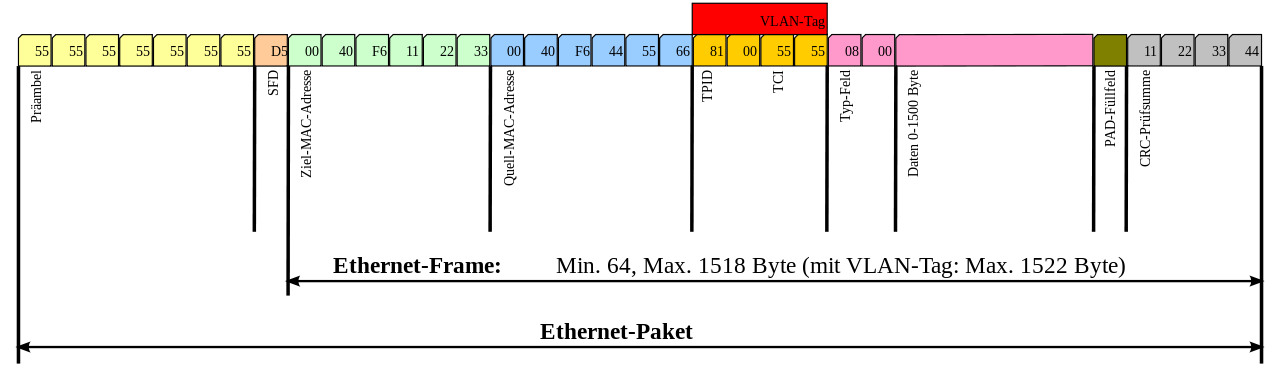
\includegraphics[scale=0.35]{pics/Ethernetpaket.png}
\begin{scriptsize}
Quelle: de.wikipedia.org/wiki/Datei:Ethernetpacket.svg
\end{scriptsize}
\end{center}

Das Frame wird serialisiert und mit dem niederwertigsten Bit zuerst übertragen. Das EthernetframeF besteht aus folgenden Teilen:
\begin{itemize}
\item Präambel und SFD\\
Dieser Teil des Paketes sind im Grunde nur Überbleibsel aus den alten Tagen. Die Präambel hat ein alternierendes Bitmuster über 7 Byte, während der SFD (Start Frame Delimeter) das Muster 10101011 trägt.\\
Diese Felder wurden früher benötigt, um den einzelnen Devices eine Möglichkeit zu geben, sich auf die Bitabstände zu synchronisieren.\\
Die große Länge der Präambel liegt darin begründet, dass beim Passieren eines Repeaters oder Hubs immer ein Teil verloren ging. Um zu gewährleisten, dass auch bei maximal großen Netzwerken die Devices noch ein Minimum an Zeit haben sich zu synchronisieren, wurde die Länge auf 7 Bytes festgesetzt. 
\item Source- und Destination MAC-Adresse\\
Stehen für Quelle des Paketes und Empfänger des Paketes (siehe Kapitel \ref{sssec:macaddr} auf Seite \pageref{sssec:macaddr})
\item VLAN-Tag\\
Der VLAN-Tag ermöglicht das Auseinanderhalten von verschiedenen VLANs (siehe Kapitel \ref{sssec:vlan} auf Seite \pageref{sssec:vlan})
\item Typ Feld\\
Das Typ Feld oder EtherType Feld legt fest, welches Protokoll sich in der Payload befindet. So steht zum Beispiel der Wert 0x0800 für IP oder 0x0806 für ARP.
\item Payload\\
Die Payload oder Nutzlast ist die Nachricht, die das Ethernetframe mit sich nimmt. Diese kann nicht größer als 1500 bytes sein.
\item Pad bytes\\
Die Pad oder Padding bytes sind dazu da, das Ethernet Paket auf eine minimale Größe von 64 bytes zu bringen, da es bei den früheren Varianten ansonsten zu Problemen mit der Collisiondetection gegeben hätte.
\item FCS Feld\\
Das FCS (Frame Check Sequence) Feld beinhaltet eine 32 bit CRC Prüfsumme welche aus den Werten des reinen Layer2 Frames besteht. Also den bits von der MAC-Adresse bis hierher.
\end{itemize}

\subsection{Address Resolution Protocol - ARP}\label{ssec:arp}
\textbf{ARP} ist ein essentielles Protokoll für die Kommunikation in einem Netzwerk. Da, damit Kommunikation stattfinden kann, die MAC-Adresse bekannt sein muss, wurde dieses Protokoll entwickelt.\\
Es funktioniert folgendermaßen: Indem ein Broadcast in das Netz geschickt wird, in welchem die Bitte steht, dass ein Host mit einer gewissen IP doch seine MAC-Adresse übermitteln soll, kann ein Rechner die benötigte Information bekommen. Diese speichert der PC, der die Anfrage gestellt hat, in seinem lokalen Cache, damit er nicht jedes Mal nachfragen muss.\\
Dieses Protokoll wird mit der Verbreitung von IPv6 aussterben, da in IPv6 das sogenannte \textbf{Neighbour Discovery Protocol NDP} diese Aufgabe übernimmt.\\

Das ARP Paket befindet sich gleichzeitig auf Layer2 und 3 und sieht wie folgt aus:\\
\begin{itemize}
\item Hardwareadresstyp\\
Die Zahl in diesem Feld bestimmt den Typen der MAC-Adresse. Dies ist meistens Ethernet, was mit einer 1 repräsentiert wird.
\item Protokolladresstyp\\
Der Adresstyp für den die MAC-Adresse angefordert wird. Im Falle von IP ist dies 0x0800. Die Zahlen in diesem Feld teilen sich ihre Nummern mit dem EtherType beim Ethernet Protokoll.
\item Hardwareadresslänge\\
Die Länge der aufgelösten Adresse. Für Ethernet ist sie 6.
\item Protokolladresslänge\\
Die Länge der Adresse, die aufgelöst werden soll. Für IPv4 lautet sie 4.
\item Operation\\
Enthält eine Zahl, die angibt, ob das Paket ein Request (1) oder eine Response (2) ist.
\item Quell MAC-Adresse
\item Quell IP-Adresse
\item Ziel MAC-Adresse\\
Enthält FF:FF:FF:FF:FF:FF, die Layer2 Broadcast Adresse.
\item Ziel IP-Adresse
\end{itemize}
Es gibt jedoch auch noch andere Arten von ARP Paketen. Dazu zählen der Reverse ARP, welcher die MAC- in eine IP-Adresse auflösen kann oder der Gratuitos ARP, welcher eine Nachricht darstellt, die unaufgefordert bekannt macht, welche MAC-Adresse man selbst hat.
\subsection{Internet Protocol - IP}\label{ssec:ip}
Das \textbf{Internet Protokoll} hat zwei Hauptaufgaben:
\begin{itemize}
\item \textbf{Adressierung}\\
Das Ziel der Adressierung auf dieser Ebene ist es, wie bereits zuvor besprochen, ein Gerät über mehrere Netzwerke hinweg eindeutig zu machen, um Pakete nicht nur innerhalb eines Netzwerkes sondern über mehrere Netzwerke hinweg ansprechen zu können.
\item \textbf{Fragmentierung}\\
Da Kommunikation sich ja meistens nicht mit nur einem Paket ausgeht, ist es wichtig, dass Kommunikationsstränge aufgeteilt werden können in mehrere kleine Pakete. Dies nennt man dann Fragmentierung. IP ist dafür zuständig, dass fragmentierte Pakete wieder zusammenfinden können, da es ja nicht heißen muss, dass nur eine einzige Kommunikation gerade am Laufen ist.\\
Dies gilt jedoch nur mehr für IPv4, denn in IPv6 ist es nicht mehr vorgesehen, dass Pakete fragmentieren.
\end{itemize}
\subsubsection{IPv4}
IP Version 4 war der erste offizielle Standard des Internet Protocols.\\
Adressierung im Schema von IPv4 wurde bereits in Kapitel \ref{sssec:ipaddr} auf Seite \pageref{sssec:ipaddr} besprochen.\\

Es gibt einige gesonderte Adressbereiche in IPv4, welche nicht für die öffentliche Nutzung verwendbar sind. Dazu zählt:
\begin{itemize}
\item 10.0.0.0/8\\
Sogenanntes Class A Netz: 1 Netz mit 16.777.216 Adressen (erstreckt sich bis 10.255.255.255/8)
\item 172.16.0.0/12\\
Sogenanntes Class B Netz: 16 Netze mit jeweils 65.536 Adressen (erstreckt sich von 172.16.0.0/16 über 172.17.0.0/16 usw. bis 172.32.0.0/16)
\item 192.168.0.0/16\\
Sogenanntes Class C Netz: 256 Netze mit je 256 Adressen (erstreckt sich von 192.168.0.0/24 über 192.168.1.0/24 usw. bis 192.168.255.0/24)
\item 100.64.0.0/10\\
Der sogenannte Shared Adress Range. Er ist speziell für Internet Service Provider und ihre Anforderungen beim NAT bestimmt und nicht für den normalen User gedacht.
\item 169.254.0.0/16\\
Link Local Adressbereich. Er wird verwendet, wenn keine spezifische IP-Adresse einem Rechner zugewiesen wird. Damit sind auch zwei Clients in der Lage miteinander zu reden, wenn sie unkonfiguriert und ohne DHCP-Server entweder direkt durch Kabel oder über einen Switch verbunden sind.
\item 127.0.0.0/8\\
LoopBack. Dieser Adressbereich wird für Interfaces des Hosts selbst verwendet. 
\item ...\\
Es gibt noch einige Bereiche mehr, aber es würde hier zu weit führen alle aufzuzählen. Sie können in der RFC6890 (zum Zeitpunkt des Schreibens aktuelle Version) nachgelesen werden.
\end{itemize}

Obwohl IPv4 schon seit mehreren Jahren von IPv6 abgelöst wurde, sind bis heute die wenigsten Firmen und noch weniger Heimnetzwerke auf IPv6 umgestellt. Es wird also im Grunde noch überall IPv4 verwendet, obwohl der Adressbereich ($2^{32} = 4.294.967.296$, abzüglich reservierter Adressen = 3.707.764.736) in dieser Version bereits \textbf{vollständig aufgebraucht} ist.\\

Dieser Problematik wurde mit einigen Zwischenlösungen begegnet. Das Protokoll \textbf{NAT (Network Address Translation)} ist eines dieser Behilfsmittel.\\
Der IPv4 Standard sieht eine Aufteilung in öffentliche und private Netzwerke vor. Adressen, welche aus dem Bereich der Privaten Netzwerke kommen, müssen nicht eindeutig sein und können so oft wie gewünscht verwendet werden. Durch ihre Mehrdeutigkeit sind sie jedoch auch nicht dazu geeignet, im Internet verwendet zu werden, sondern sie sind für den privaten Gebrauch gedacht, daher auch Privates Netzwerk.\\
Will man nun aus seinem privaten Netz raus in das Internet, wendet jener Router, welcher das private Netz mit dem des Providers verbindet, NAT an.\\
Er legt dabei eine Tabelle an, in welcher die private Adresse sowie der Port steht, und ersetzt diese durch eine öffentliche Adresse und einen beliebigen anderen High Port. Die Antworten weist er anhand des Ports dann wieder der richtigen privaten Adresse zu und leitet diese vom Internet zu dem Host, der die Anfrage abschickte.\\
Dadurch scheint es, als würden mehrere Hosts die gleiche IP-Adresse haben, nämlich jeder, welcher über diesen Router das private Netzwerk verlässt.\\

Eine andere Art, mit der das unausweichliche Versiegen an Adressen versucht wurde hinauszuzögern, ist die \textbf{dynamische Adressenvergabe von Providern an ihre Kunden}.\\
Sieht man sich mithilfe von externen Tools die Adresse, welche man nach außen hat, an zwei verschiedenen Tagen an, kann es sein, dass sich diese unterscheiden.\\
Der Provider verwendet diese Methode, um mehrere Kunden mit Adressen zu versorgen, als er eigentlich hat. Er geht dabei davon aus, dass zu keiner Zeit alle seine Kunden gleichzeitig online sind.\\

Das Problem entwickelte sich daraus, dass anfangs die Meinung geläufig war, es seien weitaus genug Adressen verfügbar. Deshalb hat man große Adressbereiche billig an Universitäten und Organisationen oder Firmen verkauft, ohne einen Gedanken daran zu verschwenden, dass womöglich irgendwann keine Adressen mehr übrig sein könnten.\\
Offiziell wurden im \textbf{Januar 2011} die letzten beiden verfügbaren IPv4 Netze der RIR (Regional Internet Registry) von der IANA (Internet Assigned Numbers Authority) zugewiesen, welche diese nun an die einzelnen Länder aufteilen.\\

Warum die Verwendung des IPv6 Standards trotzdem soweit hinausgezögert wird, liegt an der Starre der Firmen. Die Umstellung auf IPv6 bedeutet viele Probleme, da, obwohl er bereits von fast jeglicher Hardware unterstützt, immer noch Kompatibilitätsprobleme mit sich bringt. Firmen sehen keinen Sinn darin viel Geld zu investieren, um etwas zu implementieren, was doch sowieso funktioniert.\\

Der IP-Header sieht wie folgt aus:\\
\begin{center}
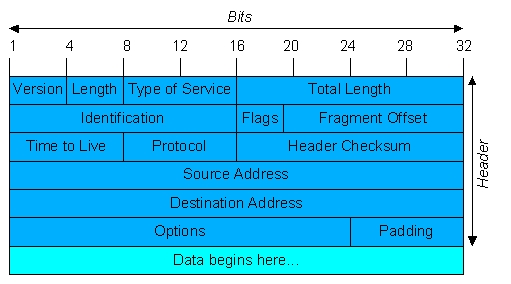
\includegraphics[scale=1]{pics/ipheader.jpg}
\begin{scriptsize}
www.rvs.uni-bielefeld.de/~heiko/tcpip/tcpip\_html\_alt/kap\_2\_3.htm
\end{scriptsize}
\end{center}
\subsubsection{IPv6}
IPv6 ist der offizielle Nachfolger von IPv4. Er ist seit 1998 von der IETF standardisiert und bringt einige Neuerungen in das Internet Protocol welche die Fehler, die durch das unterschätzte Wachstum des Internets hervorgerufen wurden, aufheben soll.\\

Eine dieser Neuerungen, wahrscheinlich auch die wichtigste, ist der \textbf{vergrößerte Adressbereich}. Während IPv4 $2^{32}$, also etwas mehr als 4 Milliarden Adressen hat, verfügt IPv6 über $2^{128}$, umgerechnet über 340 Sextillionen oder $3,4 \cdot 10^{38}$ Adressen.\\
Ein anschaulicheres Beispiel bietet folgender Vergleich: Das Alter der Erde wird auf etwa 4,5 Milliarden Jahre geschätzt. Hätte man gleichzeitig mit der Entstehung der Erde begonnen mit einer Rate von 1 Milliarde Adressen pro Sekunde IPv6 Adressen aus dem vorhandenen Adressraum zu verteilen, wäre bis heute nur weniger als ein Billionstel des vorhandenen Adressraums vergeben.\\
Damit dürfte das Problem des Adressenmangels vorübergehend gelöst sein.\\

Weitere Vorteile sind das Anpassen der Headers an die neuen Anforderungen.\\
So ist beispielsweise IPsec bereits im IPv6 selbst implementiert. Auch der Rechenaufwand für Router soll damit minimiert werden.\\

Eine Aufgabe, die IPv6 nicht länger vollbringt, wird das zuvor erwähnte Fragmentieren sein. Wenn ein Router ein Paket bekommt, welches größer ist als sein MTU (Maximal Transition Unit), verwirft er das Paket und sendet ein ICMPv6 Paket mit der Meldung \glqq Too Big\grqq . Es ist nun die Aufgabe der Schichten darüber dafür zu sorgen, dass die Pakete, welche sie versenden wollen, nicht zu groß sind.\\

Die Adressnotation in IPv6 ist deutlich anders als bei IPv4. Es gibt aufgrund der Länge und schweren Handhabbarkeit der Adressen einige Vereinfachungsregeln, welche darauf abzielen, die Adressen zu kürzen. Da die Adressen sehr viel länger sind, kommt eine dezimale Notation, wie sie vorher Verwendung fand, nicht mehr in Frage.\\
IPv6 verwendet daher Hexadezimale Notation, teilt die Adresse in 8 Blöcke auf und fasst in jedem Block 16 bit (=4 Hexadezimalstellen) zusammen. Die Blöcke werden durch Doppelpunkte getrennt: \textbf{2001:0db8:85a3:08d3:2219:8a2e:0370:7344}\\
Führende Nullen dürfen dabei ausgelassen werden.\\ \textbf{2001:0db8:85a3:08d3:0000:8a2e:0070:7344} entspricht also\\ \textbf{2001:db8:85a3:8d3:0:8a2e:70:7344}\\
Kontinuierliche Blöcke aus 0 dürfen komplett ausgelassen und durch einen zweifachen Doppelpunkt angezeigt werden. Diese Maßnahme darf jedoch nur einmal Verwendung finden, da es sonst zu Mehrdeutigkeiten kommen kann. Beispiel: \textbf{2001:0db8:85a3:0:0:8a2e:0:0} darf entweder als \textbf{2001:0db8:85a3::8a2e:0:0} oder als \textbf{2001:0db8:85a3:0:0:8a2e::} geschrieben werden.\\

Die \textbf{128 bit} lange Adresse wird in \textbf{zwei 64 bit} große Teile aufgeteilt. Ersterer ist der sogenannte \textbf{Präfix}.\\
Die letzten 64 bit jedoch sind der für jede Netzwerkschnittstelle eindeutige \textbf{Network-Identifier}. Dieser wird anhand der MAC-Adresse ausgerechnet.\\
Daraufhin wurde Kritik aus der Internetgemeinde laut, da so die Anonymität des Internets vollständig verloren gehen würde. Die IETF hat daraufhin mit der RFC4941 die \textbf{Privacy Extensions} eingeführt, welche den Host selbstständig zufällig generierte Network Identifiers machen lässt. Dieser ist in den meisten Betriebssystemen standardmäßig aktiv.\\
Dies erhöht die Anonymität zwar, reicht aber noch nicht, solang der Präfix, welcher meistens vom ISP vorgegeben wird, ebenso eindeutig ist. Sollte dieser ebenso dynamisch vergeben werden, ist ein guter Teil der Anonymität, welche IPv4 hatte, wieder gegeben.\\

Wenn eine IPv6 Adresse als URL verwendet werden soll, wird sie in eckige Klammern geschrieben, damit einer Verwechslung mit der Portnummer als Teil der Adresse vorgebeugt wird.\\

Da es keine privaten Netze mehr gibt, fallen viele reservierte Adressbereiche weg. Ein paar Wesentliche sollen trotzdem genannt werden:
\begin{itemize}
\item ::1/128\\
Die LoopBack Adresse, entspricht 127.0.0.1 bei IPv4
\item fe80::/10\\
Link Local, entspricht 169.254.0.0 bei IPv4, wird verwendet für die Neighbour-Discovery und Autoadresszuweisungen.
\item 2000::/3 - 3fff::/3\\
Momentaner Bereich für global eindeutige Adressen.
\item 2001::\\
Werden den ISPs für ihre Kunden gegeben.
\item 2001:0db8::/32\\
Für Dokumentationszwecke
\item ...\\
Auch hier kann wieder in der RFC 6890 nachgelesen werden, um mehr zu erfahren.
\end{itemize}
\subsection{Internet Control Message Protocol - ICMP}
Das Internet Control Message Protocol bewegt sich auf Layer 3 zusammen mit IP. Es dient dazu, anderen Geräten \textbf{Informationen über ihren Status} zukommen zu lassen. Es gibt eine Variante für IPv6, das sogenannte ICMPv6. Es verwendet zum Transport IP, obwohl es auf dem gleichen Layer liegt, da es sich als ein Protokoll höherer Ebene interpretiert.\\

Der Header des ICMP Paketes ist sehr klein. Er besteht lediglich aus:
\begin{itemize}
\item Type\\
Stellt die Art des ICMP dar. Kann zB. 3 für \glqq Ziel nicht erreichbar\grqq \ sein.
\item Code\\
Bietet eine genauere Auflösung der Art. Wenn der Typ zB. 3 ist, gibt es die Codes 0 für \glqq Netzwerk nicht erreichbar\grqq , 1 für \glqq Host nicht erreichbar\grqq , 2 für \glqq Protokoll nicht erreichbar\grqq \ und noch einige andere.
\item Checksum
\item Daten
\end{itemize}

Wichtige Beispiele für die Funktionen dieses Protokolls sind die Meldungen \textbf{Host Unreachable} oder \textbf{Destination Port Unreachable} für die Berichterstattung, es gibt aber auch Analysefunktionen wie traceroute oder den ICMP Echo Request. 
\paragraph{Echo Request/Response - Ping}
Der ICMP Echo hat die Typen Nummer 0. Er wurde durch das \textbf{Netzwerkprogramm Ping} auch unter diesem Namen bekannt.\\
Es wird verwendet um zu überprüfen, ob ein gewisser Host im Netzwerk ist oder nicht. Wenn ein Host ein Echo Paket empfängt, antwortet er mit einem Response Paket, genannt Pong.\\

Die Namensgebung kommt vom Sonar in U-Booten, die jedes Mal ein Ping von sich geben, wenn sie ihre Schallwellen aussenden, und ein Pong, wenn die Schallwellen von etwas reflektiert werden.\\ 
Gleich wie beim Sonar kann aus dem Echo Paket einiges an Information ausgelesen werden. So gut wie immer ist die Round-Trip Time, also die Zeit, die ein Paket benötigt, um vom Sender zum Ziel und wieder zurück zu kommen, dabei sowie der Wert aus dem Time To Live Feld, also wie viele Hops es noch passieren kann, bevor es verworfen wird.
\subsection{File Transport Protocol - FTP}
Das File Transport Protocol ist, wie der Name schon sagt, ein Protokoll zum \textbf{Übertragen von Dateien}. Es setzt auf TCP auf, da es sich nicht erlauben kann, dass Pakete verloren gehen, weil ansonsten die gesamten Daten unbrauchbar werden können. TCP verwendet \textbf{getrennte Verbindungen} für Data Transfer und Command Transfer. FTP antwortet auf Commands mit \textbf{dreistelligen Zahlen Codes} wie 200 für OK.\\

Um eine Verbindung aufzubauen, öffnet ein Client eine TCP Verbindung zum Port 21 von einem zufälligen Port N aus. Von diesem Zeitpunkt an wird es wichtig, ob der FTP Server als \glqq aktive\grqq \ oder als \glqq passive\grqq \ betrieben wird.\\
Bei einem als aktiv konfigurierten Server wartet der Client nun auf dem Port N+1 auf eine einkommende Datenverbindung. Damit der Server weiß, auf welchen Port er die Verbindung aufbauen soll, wird in der Command Verbindung ein PORT Befehl gesendet.\\
Sollte der Server als passiv konfiguriert sein, was häufig bei Servern hinter einer Firewall gemacht wird, sendet der Client ein PASV Paket über die Command Verbindung und bekommt daraufhin vom Server eine IP und einen Port, auf welchen daraufhin die Datenverbindung aufgebaut wird.\\

Ein großes Problem von FTP ist, dass, auch wenn es durch Username und Passwort geschützt werden kann, alles in Klartext überträgt. Es ist also für einen unerwünschten Mithörer im Netzwerk nicht sehr schwer alles mitzubekommen, was zwischen FTP Client und Server an Kommunikation passiert.\\
Um dies zu umgehen gibt es einige Varianten von FTP, welche Sicherheit garantieren sollen, wie u.a. \textbf{FTPS (File Transport Protocol SSL/TLS) oder SFTP (SSH File Transport Protocol)}, welche trotz des ähnlichen Namens unterschiedlich realisiert sind. 
 
\subsection{Simple Network Managing Protocol - SNMP}
Das SNMP dient dazu, die Pakete zu beschreiben, mit welchen Informationen zwischen verschiedenen Netzwerkgeräten ausgetauscht werden können. Diese Informationen finden sich in einer \textbf{MIB}. Es setzt auf UDP auf.\\

MIBs oder Management Information Bases sind \textbf{Tabellen mit beschreibenden Werten}. Diese Werte sind in einer \textbf{Baumstruktur} angeordnet. Der für SNMP interessante Bereich beginnt bei 1.3.6.1, dem Internet Zweig. Was in der MIB steht, ist von der IETF vorgegeben. SNMP weiß jedoch nicht, mit welchem Device es gerade redet, weshalb es nur als \glqq Bote\grqq für die Informationen dient.\\
Die Informationen, welche damit abgerufen werden können, sind unglaublich vielfältig und umschließen sogar Dinge wie Fehlerpakete auf einem bestimmten Interface auf einem Host.\\

Die MIB:
\begin{center}
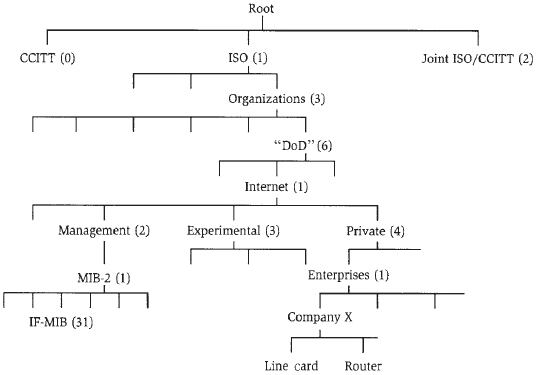
\includegraphics[scale=0.7]{pics/mib.jpg}
\begin{scriptsize}
Quelle: sourcedaddy.com/networking/images/inmg2.gif
\end{scriptsize}
\end{center}

Es gibt inzwischen \textbf{drei Versionen} von SNMP. Der Hauptkritikpunkt an den ersten Versionen war die Unsicherheit. Es ging so weit, dass im Scherz behauptet wurde, SNMP stehe eigentlich für \textbf{S}ecurity? \textbf{N}ot \textbf{m}y \textbf{P}roblem. Dies wurde auch erst mit der letzten Version, Version 3 wirklich ausgebessert.\\
Davor wurde nur mit einem sogenannten \textbf{Community String}, welches eine Art Passwort darstellt, gesichert und selbst dieser wurde in Klartext übermittelt.\\
Dies wurde in Version 3 dann verbessert und mit zwei zusätzlichen Passphrasen, genannt \textbf{Authentification und Privacy}, welche mit verschiedenen Verschlüsselungen versehen werden können, hinzugefügt wurden.\\

\begin{center}
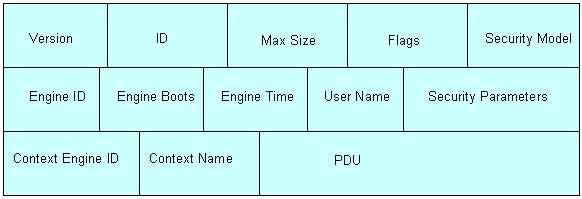
\includegraphics[scale=0.7]{pics/snmpheader.jpg}
\begin{scriptsize}
Quelle: verticalhorizions.in/wp-content/uploads/2011/09/SNMPv3\_Message\_Format.bmp
\end{scriptsize}
\end{center}

Es gibt mehrere Möglichkeiten wie SNMP Informationen aus einer MIB bekommt. Der Standard ist die \textbf{GET Methode}, bei der er ein Feld abfrägt. Doch gibt es auch die Methoden \textbf{GETNEXT und GETBULK}.\\
Bei ersterer Methode wandert er eine spezifizierte Anzahl an Werten ab. Diese Methode wurde erst in Version 2 dazugenommen.\\
Bei zweiterer Methode erfrägt er einen gesamten Unterbaum.\\

Des Weiteren gibt es noch eine Sonderform, in welcher nicht der Agent, so wird derjenige genannt, welcher die SNMP Abfragen durchführt, sondern das zu managende Device selbst sich meldet.\\
Diese sogenannten \textbf{Traps} können auf bestimmte Events gesetzt werden, wie zB. eine Änderung eines kritischen Wertes. Bei weitem öfters wird es jedoch verwendet, wenn eine der Zähler Variablen überläuft. Dabei setzen MIBs meist ein Flag in einem bestimmten Unterbaum, auf welches die Traps dann reagieren.\\

Obwohl das Protokoll sich selbst als \glqq Simple\grqq \ bezeichnet, ist es hoch komplex und, obwohl es von einem großen Teil ernstzunehmender Administratoren genutzt wird, bringt es auch extreme Sicherheitsprobleme mit, wenn man es nicht vorsichtig implementiert.\\
Vorallem die Tatsache, dass SNMPv3 Support, obwohl es ein Standard ist, so gut wie nirgends gegeben ist (unter anderem unterstützt Windows bis jetzt nur SNMPv2(c)), macht es große Probleme. 
\subsection{Hypertext Transfer Protocol - HTTP}
HTTP ist wohl eines der Protokolle, welches der Standarduser am häufigsten verwendet, auch wenn er sich dessen unter Umständen gar nicht bewusst ist. Es wird verwendet, um \textbf{Webseiten über ein Netzwerk zu transportieren}. HTTP befindet sich auf den Layern 5 bis 7 und setzt auf TCP auf, da sich vermisste oder fehlerhafte Pakete doch deutlich in der Seitendarstellung auswirken.\\
Momentan wird \textbf{HTTP/1.1} verwendet, wobei die HTTP-Entwicklergruppe der IETF bereits dabei ist, Version 2 zu spezifizieren. Ziele der neuen Version sind bessere Datenkomprimierung, effizientere Kommunikation und erhöhte Sicherheit.\\

Sicherheitstechnisch ist HTTP nicht sehr ausgefeilt. Es verwendet keine Verschlüsselung von sich aus, überträgt alles in Klartext. Dafür wurden diverse Erweiterungen geschrieben, wie zum Beispiel \textbf{HTTPS, welches Pakete mit SSL Verfahren sichert}.\\

Aufgrund diverser Erweiterungen in den Anfragenpaketen ist HTTP inzwischen über den bloßen Transport von Hypertext hinaus, es kann bereits genauso zur Übertragung von zB. Dateien verwendet werden.\\

Eine Kommunikation mit HTTP läuft immer nach einem gewissen Schema ab:\\
Ein Client schickt eine Anfrage an eine URL, wie zB. www.example.com ab. Dieser Name wird, wie bereits besprochen, über DNS aufgelöst, sollte er nicht in der hosts Datei stehen.\\
Der Webbrowser setzt an die URL normalerweise immer noch \glqq \textbackslash index.html \grqq .\\
Dies wandelt der Browser dann in ein HTTP GET Paket um, in dem neben der verwendeten HTTP Version steht, was man von welchem Client bekommen will.\\
Der Server antwortet darauf hin zuerst mit einem \textbf{Statuscode}. Dieser beschreibt, ob die Anfrage erfolgreich war oder nicht. Der Statuscode, den die meisten User kennen, ist \textbf{Error 404}, was für \textbf{Side not found} steht.\\
Ist die Anfrage jedoch erfolgreich, bekommt der Client den \textbf{Code 200} zurück, zusammen mit einigen Informationen zum Server, wie Sprache, welcher Server läuft und/oder Content type.